\documentclass[a4paper, 12pt]{article}

\usepackage{cmap}
\usepackage[T2A]{fontenc}
\usepackage[utf8]{inputenc}

\usepackage{amsmath, amsfonts, amssymb, amsthm, mathtools}
\usepackage{icomma}

\title{Отчет о выполнении лабораторной работы \\ Определение скорости полёта пули при помощи баллистического маятника}
\author{Лепарский Роман}
\date{10.11.2020}

\begin{document}

	\maketitle

	\newpage
	
	\section{Аннотация}

		Целью работы является определение скорости полёта пули при помощи баллистических маятников, применяя законы сохранения.

	\section{Теоретические сведения}

		Классический метод определения скорости, путём измерения времени пролёта пули на известное расстояние, в данном случае неуместен.
		Поскольку лабораторная установка не должна превышать нескольких метров в длину, а время пролёта пули из духовой винтовки не 
		превышает $10^{-2}$с, такое малое время можно посчитать только дорогостоящим оборудованием.

		В данном случае лучше использовать законы сохранения. Если масса тела значтельно болььше массы пули, то скорость тела с застрявшей в нем пулей будет значительно меньше скорости пули, и её будет легче измерить.

		Для измерения переданной пулей импульса и следовательно её скорости используют баллистический маятник. 
		Всилу малости отклонения такого маятника за время взаимодействия с пулей относительно амплитуды (максимального отклонения), им можно пренебречь.

		Работа состоит из двух частей:

		\subsection{Метод баллистического маятника, совершающего поступательные движения}
		
			Используемый в данной работе маятник представляет собой тяжёлый цилиндр, подвешенный на четырёх нитях одинаковой длины

			\begin{center}
			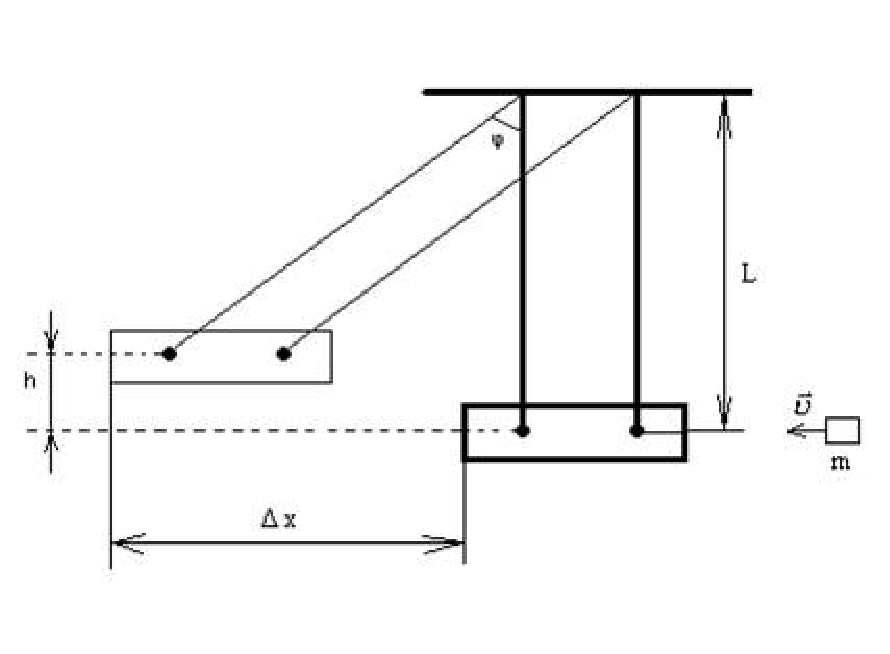
\includegraphics[scale = 0.5]{pendulum.eps}
			\end{center}

			Чтобы найти связь скорости пули и амплитуды колебаний цилиндра, воспользуемся законами сохранения:

			\begin{align*}
				mv &= (M + m)u \\
				\frac{(M + m)u^2}{2} &= 2(M + m)gh
			\end{align*}

			Высота подъема маятника выражается через угол $\varphi$ отклонения маятника от вертикали:

			\[
				h = L(1-cos(\varphi)) \approx \frac{\Delta x^2}{2L}
			\]

			Из всех этих уравнений получаем:

			\begin{equation} \label{eq:v1}
				v = \frac{M}{m}\sqrt{\frac{g}{L}}\Delta x \text{.}
			\end{equation}

		\subsection{Метод крутильного баллистического маятника}

			Схема эксперимента:

			\begin{center}
				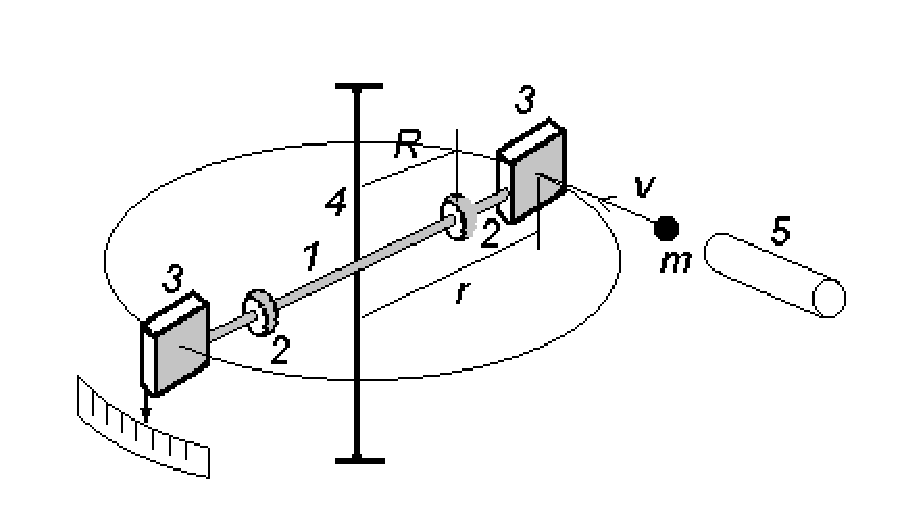
\includegraphics[scale = 0.5]{pend2.eps}
			\end{center}

			Пуля массой $m$ попадает в мишень, укреплённую на стержне, которая вместе с грузами массой $M$
			и проволокой образуют крутильный маятник. Считая удар неупругим, для определения скорости $v$ полета
			пули непосредственно перед ударом воспользуемся законом сохранения момента импульса в виде
			\begin{equation} \label{eq:moment}
				mvr = I\Omega
			\end{equation}
			Здесь $r$ - расстояние от линии полёта пули до оси вращения маятника, $I$ - момент инерции маятника, $\Omega$ - 
			его угловая скорость непосредственно после удара.

			Начальная кинетическая энергия вращения маятника переходит в потенциальную - упругую энергию закручивания проволоки.
			Пренебрегая потерями энергии, закон сохранениия энергии можно записать следуюшим образом:
			\begin{equation} \label{eq:energy}
				\frac{k\varphi^2}{2} = \frac{I\Omega^2}{2}	
			\end{equation}
			Здесь $k$ - модуль кручения проволоки, а $\varphi$ - максимальный угол поворота маятника

			Из уравнений (\ref{eq:moment}) и (\ref{eq:energy}) получаем
			\begin{equation} \label{eq:v2beg}
				v = \varphi \frac{\sqrt{kI}}{mr}
			\end{equation}

			Угол максимального закручивания маятника в данных опытах мал и легко находится по смещению $x$ изображения нити осветителя на измерительной шкале:
			\[
				\varphi \approx \frac{x}{2d}
			\]
			Здесь $d$ - расстояние от шкалы до оси вращения маятника.

			В формулу (\ref{eq:v2beg}) входит произведение $kI$, которое можно найти по измерениям периодов колебаний маятника с грузами и 
			без них. В первом случае период равен
			\[
				T_1 = 2\pi\sqrt{\frac{I}{k}}
			\]
			Во втором
			\[
				T_2 = 2\pi\sqrt{\frac{I-2MR^2}{k}}
			\]
			Отсюда
			\[
				\sqrt{kI} = \frac{4\pi MR^2T_1}{T_1^2 - T_2^2}
			\]
			Здесь $R$ - расстояние от центров масс грузов.

			Итого:
			\begin{equation} \label{eq:v2}
				v = \frac{x4\pi MR^2T_1}{(T_1^2 - T_2^2)2dmr}
			\end{equation}

	\section{Приборы и материалы}

		\begin{itemize}
			\item Духовое ружъе на штативе,
			\item Осветитель,
			\item Оптическая система для измерения отклонений маятника,
			\item Измерительная линейка,
			\item Пули,
			\item Весы для их взвешивания,
			\item Баллистические маятники.
		\end{itemize}

	\section{Обработка результатов}

		\subsection{Метод баллистического маятника, совершающего поступательные движения}

			Данные установки:
			\begin{itemize}
				\item $L = 2245$ мм
				\item $M = 2095 \pm 5$ г
			\end{itemize}

			Составим таблицу $m$, $\Delta x$. Посчитаем $v$ по формуле (\ref{eq:v1}), занесём значения в таблицу:
			\begin{center}
				\begin{tabular}{|c|c|c|}
					\hline
					$m$, г & $\Delta x$, мм & $v$, м/с \\ \hline
					0,498  & 11,0           & 158,44   \\ \hline
					0,504  & 11,0           & 156,55   \\ \hline
					0,514  & 10,9           & 152,33   \\ \hline
					0,509  & 11,9           & 165,75   \\ \hline
				\end{tabular}
			\end{center}

			Посчитаем среднюю скорость и погрешность:
			\[
				\left<v\right> = \frac{1}{N}\sum_{i = 1}^N v_i = 158,27 \text{ м/с}
			\]
			\[
				\sigma = \sqrt{\frac{1}{N}\sum_{i = 1}^N (\left<v\right> - v_i)^2} = 4,9 \text{ м/с}
			\]

		\subsection{Метод крутильного баллистического маятника}

			Данные установки:
			\begin{itemize}
				\item $d = 345$ мм
				\item $M = 714 \pm 0,1$ г
				\item $R = 340$ мм
				\item $r = 210$ мм
				\item $T_1 = 17$ с
				\item $T_2 = 10,4$ с
			\end{itemize}

			Составим таблицу $m$, $x$. Посчитаем $v$ по формуле (\ref{eq:v2}), занесём значения в таблицу:
			\begin{center}
				\begin{tabular}{|c|c|c|}
					\hline
					$m$, г & $x$, см & $v$, м/с \\ \hline
					0,507  & 9,5     & 139,36   \\ \hline
					0,504  & 8,2     & 122,83   \\ \hline
					0,507  & 9,0     & 132,72   \\ \hline
					0,503  & 8,5     & 127,09   \\ \hline
				\end{tabular}
			\end{center}

			Посчитаем среднюю скорость и погрешность:
			\[
				\left<v\right> = \frac{1}{N}\sum_{i = 1}^N v_i = 130,5 \text{ м/с}
			\]
			\[
				\sigma = \sqrt{\frac{1}{N}\sum_{i = 1}^N (\left<v\right> - v_i)^2} = 6,2 \text{ м/с}
			\]

	\section{Вывод}

	Проведя измерения и обсчитав результаты, мы нашли скорость вылета пули. В 1 эксперименте $v = 158,3 \pm 4,9$ м/с, во 
	2 эксперименте $v = 130,5 \pm 6,2$ м/с. Несовпадение результатов первого и второго опыта может быть обусловлено тем,
	что в экспериментах использовались разные винтовки.

\end{document}